\section{27 Nov 23 - Notes: Counting and
Combinatorics}\label{nov-23---notes-counting-and-combinatorics}

As we discussed, \href{https://en.wikipedia.org/wiki/Entropy}{entropy}
is a fundamental concept that quantifies the degree of disorder or
randomness in a system. It was initially introduced in the mid-19th
century in the field of
\href{https://en.wikipedia.org/wiki/Thermodynamics}{thermodynamics} by
Rudolf Clausius, entropy was a measure of the unavailability of a
system's energy to do work.

\subsection{Statistical Mechanics and
Combinatorics}\label{statistical-mechanics-and-combinatorics}

In
\href{https://en.wikipedia.org/wiki/Statistical_mechanics}{statistical
mechanics}, developed by Ludwig Boltzmann and J. Willard Gibbs, entropy
was redefined as a measure of uncertainty or information about a system.
This brings in the concept of entropy as a measure of the number of
possible microstates (specific arrangements of particles) corresponding
to a macrostate (the observable state of the system). As it goes, the
more microstates there are, the higher the entropy, and hence, the
greater the disorder. This is an over-simplification of what is a
fundamentally complex and interesting set of processes. This
interpretation does bridge thermodynamics with statistical mechanics,
offering a deeper understanding of temperature, pressure, and phase
transitions in terms of atomic or molecular behavior as we will see with
\href{https://en.wikipedia.org/wiki/Ideal_gas_law}{the ideal gas law}
and the \href{https://en.wikipedia.org/wiki/Ising_model}{Ising model}.

As we transition from a conceptual understanding of entropy to its
mathematical formulation, combinatorics plays a crucial role.
\href{https://en.wikipedia.org/wiki/Combinatorics}{Combinatorics} is the
branch of mathematics dealing with combinations and arrangements of
objects, becomes essential in quantifying the number of microstates in a
system. For instance, the concept of permutations and combinations helps
in counting the possible arrangements of particles under given
constraints, which is fundamental in calculating entropy.

In statistical mechanics, the number of microstates (\(\Omega\)) is
directly used in Boltzmann's entropy formula,

\[S = k \log(\Omega),\]

where \(k\) is Boltzmann's constant. This formula encapsulates the idea
that entropy is a measure of the logarithm of the number of ways in
which a system can be arranged. The combinatorial approach in
statistical mechanics provides a quantitative method to explore how
microscopic properties (like the positions and velocities of particles)
lead to macroscopic phenomena (like temperature and pressure) through
the lens of entropy.

\subsection{Fundamentals of Combinatorics and
Counting}\label{fundamentals-of-combinatorics-and-counting}

We have to learn to count microstates and do that efficiently. These
calculations will underlie a lot of the fundamentals to the statistical
mechanics we will be doing. We will start with the basics of counting
and combinatorics, which will be the foundation for understanding
entropy and statistical mechanics. We will separate this into
permutations (where the objects are distinguishable) and combinations
(where the objects are indistinguishable).

\subsubsection{Permutations (Distinguishable
Counting)}\label{permutations-distinguishable-counting}

Permutations are arrangements of objects where the order matters. You
have to be able to tell the difference between every object. For
example, you might be wanting to determine the ways you can arrange 5
balls that are all different colors. \emph{We get this is contrived, but
it's helpful to illustrate} Well, there are five ways to pick the first
ball, four ways to pick the second ball, three ways to pick the third
ball, two ways to pick the fourth ball, and one way to pick the fifth
ball. This gives us a total of 120 ways to arrange 5 balls. We can
summarize this with \(\Omega\) = number of ways,

\[\Omega(n) = n!\]

This \href{https://en.wikipedia.org/wiki/Factorial}{factorial} function
is the product of all positive integers up to \(n\). For example,
\(5! = 5 \times 4 \times 3 \times 2 \times 1 = 120\).

\subsubsection{Choosing a subset (Distinguishable
Counting)}\label{choosing-a-subset-distinguishable-counting}

What if you are trying to choose a subset of these distinguishable
objects? For example, you want to find the number of ways you can pick 3
of these objects out. Well there's five ways to pick the first object,
four ways to pick the second object, and three ways to pick the third
object. This gives us a total of 60 distinct ways to pick 3 items from 5
objects where the order matters.

But can we better quantify that process. If we have \(n\) objects and we
want to choose \(k\) objects, we can write this as,

\[\Omega(n,k) = \frac{n!}{(n-k)!}\]

Let's see that this works for our choices. We can make a table for all
the potential choices of \(k\). For \(n=5\) objects, we can pick \(k\)
of them in \(\Omega(5,k)\) ways.

\begin{longtable}[]{@{}ll@{}}
\toprule\noalign{}
k & \(\Omega(5,k)\) \\
\midrule\noalign{}
\endhead
\bottomrule\noalign{}
\endlastfoot
1 & 5 \\
2 & 20 \\
3 & 60 \\
4 & 120 \\
5 & 120 \\
\end{longtable}

\emph{Note that these numbers can get really big and cause issues with
overflow.} Sometimes you have to be careful how you form your
calculations or store your numerical variables.

\paragraph{Lecture Video}\label{lecture-video}

\href{https://inv.tux.pizza/channel/UC5KbWmC93TBhinPLqh5j2kg}{Johnathan
Gardner} has a nice set of videos on Thermodynamics and Statistical
Mechanics. Below is short one on counting and combinatorics.

\href{https://inv.tux.pizza/watch?v=tEQFftB1Pao}{\pandocbounded{\includegraphics[keepaspectratio,alt={Permutations and Combinations}]{https://markdown-videos-api.jorgenkh.no/youtube/tEQFftB1Pao?width=720&height=405}}}

\begin{itemize}
\tightlist
\item
  Non-Commercial Link: \url{https://inv.tux.pizza/watch?v=tEQFftB1Pao}
\item
  Commercial Link: \url{https://youtube.com/watch?v=tEQFftB1Pao}
\end{itemize}

\subsubsection{Combinations (Indistinguishable
Counting)}\label{combinations-indistinguishable-counting}

In statistical mechanics, our work is typically different from simple
permutations. We are often interested in the arrangement of some
important quantity (like energy) over the different bodies (atoms,
molecules, etc) in the system. Here you can think of having a bunch of
balls, each corresponding to an energy quantum. What we want to do is
arrange those quanta over different bodies, put each ball into a bin.

For example, for the
\href{https://en.wikipedia.org/wiki/Quantum_harmonic_oscillator}{quantum
harmonic oscillator}, we have a bunch of energy quanta that we want to
arrange over the different energy levels. We don't care about the order
of the energy quanta, just the number of quanta in each energy level.
This is where combinations come in. For a system with 3 atoms, we don't
care which atom is in which state, just that we know which states the
collections of atoms are in. So

Because ultimately, it's the combination of how the energy are
distributed that determine the system's state. it's not how each quanta
are distributed on each atom, molecule, or body. Let's do an example.
Suppose we have \(q=5\) quanta of energy to distribute amongst \(N=2\)
oscillators (think of them as atoms being put into a particular energy
state). We can write down all the possible states if we use the pair of
numbers (\(N_1\), \(N_2\)) to denote the number of quanta in each
oscillator. For example, (3, 2) means that oscillator 1 has 3 quanta of
energy and oscillator 2 has 2 quanta of energy. We could write down all
the possible states and count them up, but that's definitely not
efficient, nor do we care about the order of the quanta.

\subsubsection{Derivation of the Einstein Counting
Formula}\label{derivation-of-the-einstein-counting-formula}

The problem we set up is a classic one in statistical physics. It was
originally attributed to Einstein. In fact the concept of an
\href{https://en.wikipedia.org/wiki/Einstein_solid}{Einstein solid}
continues to be used. It is a model of a solid based on two assumptions:

\begin{enumerate}
\def\labelenumi{\arabic{enumi}.}
\tightlist
\item
  Each atom in the solid is an independent 3D quantum harmonic
  oscillator.
\item
  All atoms oscillate with the same frequency.
\end{enumerate}

The first assumption is a good one. The second one is not. But it's a
good approximation for many solids. If we model the quanta as stars and
the oscillators as lines. Where the lines separate the stars into bins.
This is the so called
\href{https://en.wikipedia.org/wiki/Stars_and_bars_(combinatorics)}{Stars
and bars model}. We avoid that language because in the US because it
associated with a Southern hate group. In any event, here's an image to
make sense of the model:

\begin{figure}
\centering
\pandocbounded{\includegraphics[keepaspectratio,alt={Cookies given to friends}]{https://upload.wikimedia.org/wikipedia/commons/thumb/b/ba/Colored_circle_starsbars_1.svg/566px-Colored_circle_starsbars_1.svg.png}}
\caption{Cookies given to friends}
\end{figure}

We can show that the total number of symbols we have is \(q+N-1\), we
get the \(N-1\) because we need one less line to make a two bins. We can
then write down the number of ways to arrange the symbols as,

\[\Omega(q,N) = \frac{(q+N-1)!}{q!(N-1)!}\]

where the denominator is the number of ways to arrange the \(q\) quanta
(stars) and the \(N-1\) lines (or \(N\) oscillators) separately. We can
apply this model to a solid to compute the number of potential
microstates for a given macrostate.

\paragraph{Lecture Video}\label{lecture-video-1}

The video below does precisely that.

\href{https://inv.tux.pizza/watch?v=71fk3n88t48}{\pandocbounded{\includegraphics[keepaspectratio,alt={The Einstein Model of a Solid}]{https://markdown-videos-api.jorgenkh.no/youtube/71fk3n88t48?width=720&height=405}}}

\begin{itemize}
\tightlist
\item
  Non-Commercial Link: \url{https://inv.tux.pizza/watch?v=71fk3n88t48}
\item
  Commercial Link: \url{https://youtube.com/watch?v=71fk3n88t48}
\end{itemize}

\subsubsection{Example: The Einstein Model of a small
solid}\label{example-the-einstein-model-of-a-small-solid}

Consider an Einstein solid consisting of 5 atoms, 15 oscillators. Let's
allow ourselves to have 20 quantum of energy to distribute amongst the
oscillators. How many microstates are there for this system? We can use
the formula above to calculate this. But better yet, let's use Python to
calculate and display the results.

Here \(N=15\), but \(q\) is anywhere from 0 to 20. So we will need to
loop through and calculate.

\begin{Shaded}
\begin{Highlighting}[]
\ImportTok{import}\NormalTok{ matplotlib.pyplot }\ImportTok{as}\NormalTok{ plt}
\ImportTok{import}\NormalTok{ numpy }\ImportTok{as}\NormalTok{ np}

\ImportTok{from}\NormalTok{ math }\ImportTok{import}\NormalTok{ factorial}

\KeywordTok{def}\NormalTok{ calculate\_microstates(quanta, oscillators):}
    \CommentTok{"""}
\CommentTok{    Calculate the number of microstates for an Einstein solid.}
\CommentTok{    quanta: Number of quanta of energy.}
\CommentTok{    oscillators: Number of oscillators.}
\CommentTok{    returns the number of microstates.}
\CommentTok{    """}
    \ControlFlowTok{return}\NormalTok{ factorial(quanta }\OperatorTok{+}\NormalTok{ oscillators }\OperatorTok{{-}} \DecValTok{1}\NormalTok{) }\OperatorTok{/}\NormalTok{ (factorial(quanta) }\OperatorTok{*}\NormalTok{ factorial(oscillators }\OperatorTok{{-}} \DecValTok{1}\NormalTok{))}

\CommentTok{\# Number of quanta and oscillators}
\NormalTok{quanta }\OperatorTok{=} \DecValTok{20}
\NormalTok{oscillators }\OperatorTok{=} \DecValTok{15}

\CommentTok{\# Calculate the number of microstates for a range of quanta values}
\NormalTok{quanta\_values }\OperatorTok{=}\NormalTok{ np.arange(}\DecValTok{0}\NormalTok{, quanta }\OperatorTok{+} \DecValTok{1}\NormalTok{)}
\NormalTok{num\_microstates }\OperatorTok{=}\NormalTok{ [calculate\_microstates(q, oscillators) }\ControlFlowTok{for}\NormalTok{ q }\KeywordTok{in}\NormalTok{ quanta\_values]}
\end{Highlighting}
\end{Shaded}

\begin{Shaded}
\begin{Highlighting}[]
\CommentTok{\# Create a figure with two subplots}
\NormalTok{fig, (ax1, ax2) }\OperatorTok{=}\NormalTok{ plt.subplots(}\DecValTok{1}\NormalTok{, }\DecValTok{2}\NormalTok{, figsize}\OperatorTok{=}\NormalTok{(}\DecValTok{12}\NormalTok{, }\DecValTok{5}\NormalTok{))}

\CommentTok{\# Plot the number of microstates in normal scale}
\NormalTok{ax1.plot(quanta\_values, num\_microstates, marker}\OperatorTok{=}\StringTok{\textquotesingle{}o\textquotesingle{}}\NormalTok{, linestyle}\OperatorTok{=}\StringTok{\textquotesingle{}{-}\textquotesingle{}}\NormalTok{, color}\OperatorTok{=}\StringTok{\textquotesingle{}b\textquotesingle{}}\NormalTok{)}
\NormalTok{ax1.set\_xlabel(}\StringTok{\textquotesingle{}Number of Quanta\textquotesingle{}}\NormalTok{)}
\NormalTok{ax1.set\_ylabel(}\StringTok{\textquotesingle{}Number of Microstates\textquotesingle{}}\NormalTok{)}
\NormalTok{ax1.set\_title(}\StringTok{\textquotesingle{}Microstates (Normal Scale)\textquotesingle{}}\NormalTok{)}
\NormalTok{ax1.set\_xticks(quanta\_values[::}\DecValTok{2}\NormalTok{])}
\NormalTok{ax1.grid()}

\CommentTok{\# Plot the number of microstates in log scale}
\NormalTok{ax2.semilogy(quanta\_values, num\_microstates, marker}\OperatorTok{=}\StringTok{\textquotesingle{}o\textquotesingle{}}\NormalTok{, linestyle}\OperatorTok{=}\StringTok{\textquotesingle{}{-}\textquotesingle{}}\NormalTok{, color}\OperatorTok{=}\StringTok{\textquotesingle{}r\textquotesingle{}}\NormalTok{)}
\NormalTok{ax2.set\_xlabel(}\StringTok{\textquotesingle{}Number of Quanta\textquotesingle{}}\NormalTok{)}
\NormalTok{ax2.set\_ylabel(}\StringTok{\textquotesingle{}Number of Microstates (Log Scale)\textquotesingle{}}\NormalTok{)}
\NormalTok{ax2.set\_title(}\StringTok{\textquotesingle{}Microstates (Log Scale)\textquotesingle{}}\NormalTok{)}
\NormalTok{ax2.set\_xticks(quanta\_values[::}\DecValTok{2}\NormalTok{])}
\NormalTok{ax2.grid()}

\CommentTok{\# Adjust layout for better visualization}
\NormalTok{plt.tight\_layout()}
\end{Highlighting}
\end{Shaded}

\begin{figure}
\centering
\pandocbounded{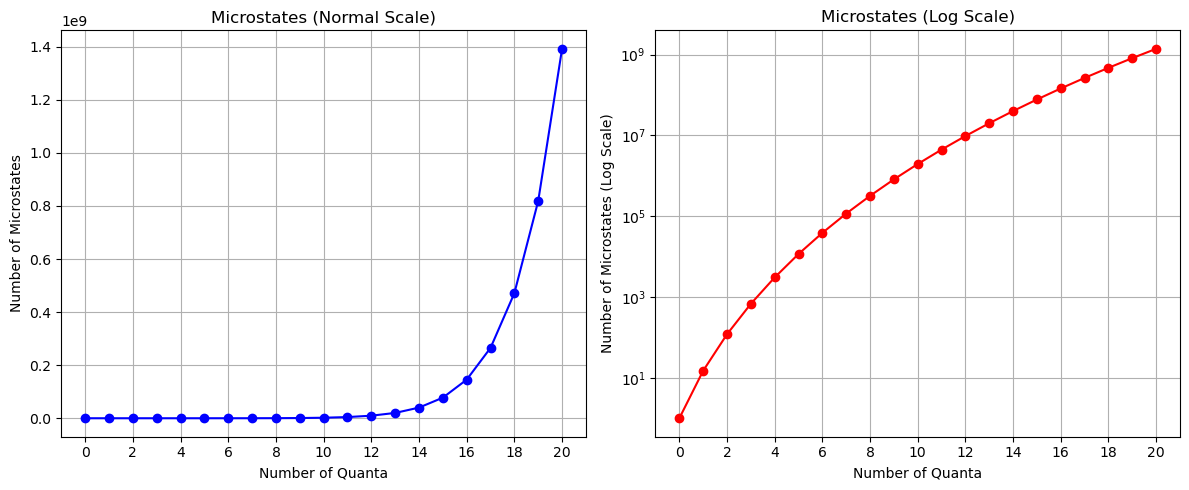
\includegraphics[keepaspectratio,alt={png}]{../images/notes-counting_and_combinatorics_notes-counting_and_combinatorics_tmp_6_0.png}}
\caption{png}
\end{figure}

\subsubsection{What about the entropy?}\label{what-about-the-entropy}

We can compute it using the formula above, but for our purposes, we will
just use the logarithm of the number of microstates.

\[S/k = \log(\Omega)\]

Notice that our log scale graph above looks exactly like the entropy
graph. The number of microstates is a measure of the entropy.

\begin{Shaded}
\begin{Highlighting}[]
\NormalTok{entropy }\OperatorTok{=}\NormalTok{ np.log(num\_microstates)}
\NormalTok{plt.plot(quanta\_values, entropy, marker}\OperatorTok{=}\StringTok{\textquotesingle{}o\textquotesingle{}}\NormalTok{, linestyle}\OperatorTok{=}\StringTok{\textquotesingle{}{-}\textquotesingle{}}\NormalTok{, color}\OperatorTok{=}\StringTok{\textquotesingle{}b\textquotesingle{}}\NormalTok{)}
\NormalTok{plt.xlabel(}\StringTok{\textquotesingle{}Number of Quanta\textquotesingle{}}\NormalTok{)}
\NormalTok{plt.ylabel(}\StringTok{\textquotesingle{}Entropy (unitless)\textquotesingle{}}\NormalTok{)}
\NormalTok{plt.xticks(quanta\_values[::}\DecValTok{2}\NormalTok{])}
\NormalTok{plt.grid()}
\NormalTok{plt.tight\_layout()}
\end{Highlighting}
\end{Shaded}

\begin{figure}
\centering
\pandocbounded{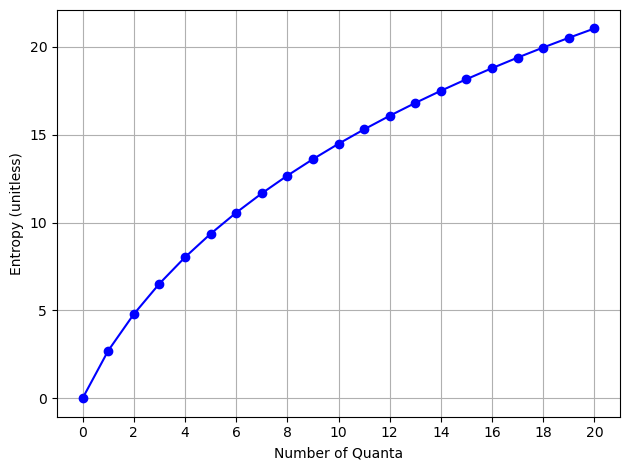
\includegraphics[keepaspectratio,alt={png}]{../images/notes-counting_and_combinatorics_notes-counting_and_combinatorics_tmp_8_0.png}}
\caption{png}
\end{figure}

\subsection{Additional Resources}\label{additional-resources}

If you want more details on combinatorics, please review this longer
lecture.

\href{https://inv.tux.pizza/watch?v=6oV3pKLgW2I}{\pandocbounded{\includegraphics[keepaspectratio,alt={Counting and Combinatorics Lecture}]{https://markdown-videos-api.jorgenkh.no/youtube/6oV3pKLgW2I?width=720&height=405}}}

\begin{itemize}
\tightlist
\item
  Non-Commercial Link: \url{https://inv.tux.pizza/watch?v=6oV3pKLgW2I}
\item
  Commercial Link: \url{https://youtube.com/watch?v=6oV3pKLgW2I}
\end{itemize}
